% -*- mode: latex; TeX-engine: xetex; LaTeX-command-style: (("" "SOURCE_DATE_EPOCH=0 %(PDF)%(latex) --shell-escape %S%(PDFout)")); TeX-master: "../dissertation.tex"; -*-

\chapter{Raman Sideband Cooling}
\label{ch:rsc}

\section{Introduction}
\label{ch:rsc:introduction}

The trapping of the single atoms in the optical tweezers in section~\ref{ch:loading:loading}
improves our control on the motional degrees of freedom of the atoms
by confining it to the focus of the tweezer.
However, the temperature of the atoms directly after loading
is still relatively high~($80~\mathrm{mK}$ for Na and
$10~\mathrm{mK}$ for Cs)
compared to the trapping frequencies~($80\sim600~\mathrm{kHz}$ or $4\sim30~\mathrm{mK}$ for Na
and $20\sim160~\mathrm{kHz}$ or $1\sim8~\mathrm{mK}$ for Cs)
of the tweazer causing a large number of motional states
to be occupied~($\approx\!60$ for Na and $\approx\!20$ for Cs).
Further cooling into the motional ground state of the tweezer for both atoms
are required in our experiment for two reasons,
\begin{enumerate}
\item Our assembly approach relies on the preparation of atomic quantum states
  to realize full control of the molecule.
  More concretely, the temperature and motional states of the molecule we create
  is directly related to the cooling of the atoms in the tweezer.
\item Cooling to the motional ground state reduces the size of the atomic wavefunction.
  This increases the interaction between the atoms and
  improves the coupling to the molecular states as will be shown in later chapters.
\end{enumerate}

The confinement provided by the optical tweezer and the relatively high trapping frequencies
enables the potential the use of Raman sideband cooling~(RSC)
in our experiment to reach the motional ground state.
Originally developed for ion systems to take advantage of the tight confinement from ion traps,
resolved sideband cooling has been later implemented for neutral atomic systems
using Raman transitions using both optical lattices and optical tweezers
on multiple species. Still, the application of RSC requires a favorable initial cooling
and very tight confinement from the trap and remains challenging and underexplored
outside this regime (formally known as the Lamb-Dicke regime,
which is defined later in section~\ref{ch:rsc:basic-theory:raman}).
The efficient polarization gradient cooling for Cs atoms allows RSC
to be implemented in a similar fashion~\cite{liu_molecular_2019} as previous experiments
achiving a ground state probability of $96(3)~\mathrm{\%}$.

Unfortunately, the parameter achievable for Na lands outside the Lamb-Dicke regime
making the implementation of RSC much more challenging.
In this chapter, we will discuss how we overcome these challanges
and achieved ground state cooling using RSC in our experiment.
We will start in section~\ref{ch:rsc:basic-theory} and \ref{ch:rsc:thermometry}
with a description of the theory for RSC and the related thermometry technique.
Section~\ref{ch:rsc:setup} describes the experimental setup for RSC.
The challenges related to cooling outside the Lambd-Dicke regime are analyzed in detail
in section~\ref{ch:rsc:challenges} followed by
section~\ref{ch:rsc:solution-high-orders} and \ref{ch:rsc:simulation}
listing the solution we developed to overcome these challenges.
The experimental realization and result of the cooling sequence
are discussed in section~\ref{ch:rsc:alignment}, \ref{ch:rsc:implementation}
and \ref{ch:rsc:performance} before the summary in section~\ref{ch:rsc:summary}.
The discussion here is based on our publication in~\cite{yu_motional-ground-state_2018}.

\section{Basic Theory}
\label{ch:rsc:basic-theory}

\begin{figure}
  \centering
  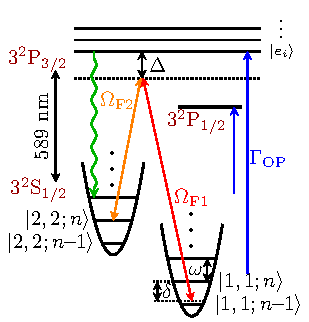
\includegraphics[width=8cm]{figures/na_rsc_schematics.pdf}
  \caption[Schematics of Raman sideband cooling for Sodium.]{
    Single Na atom Raman sideband cooling scheme.
    The Raman transitions couples $|2,2;n\rangle$ and $|1,1;n+\Delta n\rangle$
    through the intermediate states $|e_i\rangle$ in the $\mathrm{3^2P_{3/2}}$ electronic states.
    The transitions have a one-photon detuning $\Delta_i\approx75$ GHz.
    Two-photon detuning, $\delta$, is defined relative to the $\Delta n=0$ carrier transition.
    For optical pumping, we use two $\sigma^+$ polarized transitions,
    one to pump the atom state out of $|1,1\rangle$ via $\mathrm{3^2P_{3/2}}$
    and one to pump atoms out of $|2,1\rangle$ via $\mathrm{3^2P_{1/2}}$
    to minimize heating of the $|2,2\rangle$ state.
    \label{fig:rsc:na-schematics}}
\end{figure}

The relevant energy diagram and the laser frequencies for RSC are shown in
Fig.~\ref{fig:rsc:na-schematics}.
We approximate the trapping potential using a harmonic oscillator.
Since this is a separable potential, we can use only the 1D motional state $|n\rangle$
and the result can be easily generalized to the full 3D system.

The cooling sequence consists of two types of pulses.
First, a Raman pulse drives the atom to a different hyperfine state while simultaneously
reduces the motional energy of the atom.
The optical pumping~(OP) pulse afterwards then reset the hyperfine state of the atom
and reduce the entropy of the system.
This sequence is then repeated until the system reaches the ground motional state
where there is no more motional energy to be taken out of the system via the Raman pulse.
In this section, we will discuss the theory of each types of pulses individually.
We will cover how the pulses affect cooling performance in section~\ref{ch:rsc:challenges}.

\subsection{Raman Transition}
\label{ch:rsc:basic-theory:raman}

As shown in Fig.~\ref{fig:rsc:na-schematics},
the cooling sequence starts with the sodium atom in the
$|s_1\rangle\equiv|2,2\rangle$ hyperfine state,
and a Raman transition is used to drive the atom to the $|s_2\rangle\equiv|1,1\rangle$ state,
where $|F,m_F\rangle$ denotes the $F$ and $m_F$ quantum number for the sodium atom.
The full Rabi frequency for such a transition is given by~\cite{knight_quantum_2003}
\begin{align}
  \Omega_{\mathrm{R}}^0=&\sum_{i}\frac{\Omega_{1i}\Omega_{2i}^*}{2\Delta_i}\label{eq:rsc:basic-theory:raman-rabi}
\end{align}
where the sum is over all the coupled excited states,
$\Omega_{ai}\equiv\langle a|\mathbf{d}\cdot\mathbf{E}_a|e_i\rangle$ is the single photon
Rabi frequency between $|a\rangle$ and $|e_i\rangle$
and $\Delta_i$ is the single photon detuning from excited state $|e_i\rangle$.

In order to account for the motional degrees of freedom, we need to include the spatial
wavefunction of the atom and light into account.
As mentioned above, we approximate the atomic motional wavefunction by the harmonic oscillator
eigenstates $|n\rangle$. Coupling between states different $n$ states from the Raman transition
is allowed due to the recoil from the Raman lasers,
which corresponds to a spacial phase imprinting of $\ue^{\ui\mathbf{\Delta k}\cdot\mathbf{\hat x}}$
where $\mathbf{\Delta k}$ is the wavevector difference between the two Raman beams.
Using the creation~($\hat a^\dagger$) and annihilation~($\hat a$) operators and the relation
$\mathbf{\hat x}=\mathbf{x}_0\paren{\hat a+\hat a^\dagger}$ where $x_0=\sqrt{\hbar/2m\omega}$
is the harmonic oscillator length, the phase factor can be expressed as
$\ue^{\ui\eta^{\mathrm{R}}\paren{\hat a+\hat a^\dagger}}$ where $\eta^{\mathrm{R}}\equiv\mathbf{\Delta k}\cdot\mathbf{x}_0$
is the Lamb-Dicke parameter for the Raman transition.
The matrix element between motional state $|n\rangle$ and $|n'\rangle$ is therefore,
\[ M_{n,n'}=\langle n|\ue^{\ui\eta^{\mathrm{R}}\paren{\hat a+\hat a^\dagger}}|n'\rangle \]
and the final Raman Rabi frequency between motional states $n$ and $n'$ is given by,
\[ \Omega_{\mathrm{R}}^{n,n'}=M_{n,n'}\Omega_{\mathrm{R}}^0 \]
For $n=n'$, this is called a carrier transition and the others are called sideband transitions.
If the final state is higher than the initial one, i.e. $n'>n$, it is a heating sideband.
Likewise, transitions with $n'<n$ are cooling sidebands.

A closed form result for $M_{n,n'}$ is given in Ref.~\cite{wineland_experimental_1998},
\[ M_{n,n'}=\ue^{\paren{\eta^{\mathrm{R}}}^2/2}\sqrt{\frac{n_<!}{n_>!}}\paren{\eta^{\mathrm{R}}}^{|n-n'|}L_{n_<}^{|n-n'|}\paren{\paren{\eta^{\mathrm{R}}}^2} \]
where $n_<$ and $n_>$ are the lesser and greater, respectively, of $n$ and $n'$,
and $L_n^\alpha$ is the generalized Laguerre polynomial,
\[ L_n^\alpha(x)\equiv\sum_{m=0}^n(-1)^m\begin{pmatrix}n+\alpha\\n-m\end{pmatrix}\frac{x^m}{m!} \]

An important limit is the so-called Lamb-Dicke~(LD) regime defined
as $\paren{\eta^{\mathrm{R}}}^2(2n+1)\ll 1$.
In this case, we can approximate the phase factor in leading order of $\eta^{\mathrm{R}}$,
\[ \ue^{\ui\eta^{\mathrm{R}}\paren{\hat a+\hat a^\dagger}}\approx1+\ui\eta^{\mathrm{R}}\paren{\hat a+\hat a^\dagger} \]
and the matrix element
\[ M_{n,n'}\approx\delta_{n,n'}+\ui\eta^{\mathrm{R}}\sqrt{n+1}\delta_{n+1,n'}+\ui\eta^{\mathrm{R}}\sqrt{n}\delta_{n,n'+1} \]
the three terms corresponds to the carrier~($n'=n$),
the first order heating sideband~($n'=n+1$)
and the first order cooling sideband~($n'=n-1$) with corresponding strength
$1$, $\eta^{\mathrm{R}}\sqrt{n+1}$ and $\eta^{\mathrm{R}}\sqrt{n}$.
We can clearly see from this approximation that the coupling to other motional state
is stronger for a larger $\eta^{\mathrm{R}}$ and higher motional quantum number $n$.
We will discuss this effect outside the LD regime and its implication
on the cooling performance in more detail in section~\ref{ch:rsc:challenges}.

\subsubsection{Scattering from Raman Beams}
\label{ch:rsc:basic-theory:raman-scatter}

In additional to driving the Raman transition, the Raman beams can also cause scattering.
The rate of the scattering is
\footnote{Here we assume that each Raman beam only couples to their respective ground states.
  Including coupling to the other ground state increases the scattering rate but does not change
  the scaling with detuning.},
\begin{align*}
  \Gamma=&\sum_{i}\frac{\Gamma_{ei}\Omega_{1i}^2}{4\Delta_i^2}
\end{align*}
where $\Gamma_{ei}$ is the linewidth of the excited state $|e_i\rangle$.
Together with Eq.~\ref{eq:rsc:basic-theory:raman-rabi}, we see that approximately
$\Gamma/\Omega_{\mathrm{R}}\propto1/\Delta$ so a larger detuning should be used
in order to reduce the scattering during RSC.

\subsection{Optical Pumping}
\label{ch:rsc:basic-theory:op}

Driving the system on a cooling sideband with Raman transition can reduce the
motional energy of the atom. However, this is a fully coherent process that does
not reduce the system entropy and is not really ``cooling'' the system
or achieving better control on the quantum state of the system.
Instead, quantum state control is achieved in the RSC via the OP pulse.
The initial hyperfine state $|2,2\rangle$ is a stretched state so it is the
state the system naturally ends up in when $\sigma^+$ light is applied.
However, if this is done using scattering from a $F=2$ to $F'=3$ transition,
the OP beam will allow continuous photon cycle
between the $|2,2\rangle$ and the $|3',3\rangle$ causing unnecessary motional heating during OP.
Therefore, the OP must be done on a $F=2$ to $F'=2$ transition.
Unfortunately, for Na, the corresponding transition
from $\mathrm{3^2S_{1/2}}$ to $\mathrm{3^2P_{3/2}}$
that is used for the MOT is not useable due to the small energy difference of
$60 \mathrm{MHz}$~(or $6$ line widths) between the $F'=2$ and
$F'=3$ states~\cite{steck_sodium_2019}.
Instead, we must use the sodium $\mathrm{D1}$ line,
i.e. $\mathrm{3^2S_{1/2}}$ to $\mathrm{3^2P_{1/2}}$ transition,
which lacks a $F'=3$ excited state~\cite{monroe_resolved-sideband_1995,grobner_degenerate_2017}.
We find a reduction in the scattering rate by a factor of $130(20)$,
as compared to using an OP resonant with $\mathrm{3^2P_{3/2}}$.
The $\mathrm{D1}$ light with $\sigma^+$ polarization is only used to pump atoms from
$F=2$ states (in particular $|2,1\rangle$ which is populated during the OP process).
Since the goal of the OP pulse is to clear the atom population in all states but $|2,2\rangle$,
the photon cycling is not a concern for $F=1$ states and the $\mathrm{D2}$ line
is used for OP of $F=1$ states instead.
This also allow us to reuse the MOT light source and simplifies our setup.

\section{Raman Sideband Thermometry}
\label{ch:rsc:thermometry}

From the discussion in section~\ref{ch:rsc:basic-theory:raman},
we see that the strength of the sideband transition depends on the initial motional state
as well as the Lamb-Dicke parameter $\eta^{\mathrm{R}}$ of the atom.
This dependency allows us to infer the motional state of the atom
by measuring the sideband height, i.e. the so-called
sideband thermometry~\cite{monroe_resolved-sideband_1995,meekhof_generation_1996}.

In particular, for atom with temperature $T$,
the probability for the atom to be in motional state $|n\rangle$ is,
\[ p_n=\paren{1-\ue^{-\hbar\omega/k_BT}}\ue^{-n\hbar\omega/k_BT} \]
for a Raman pulse with full Rabi frequency $\Omega_{\mathrm{R}}^0$ and time $t$,
the peak height for the first order heating~(+) and cooling~(-) sidebands,
\begin{align*}
  h_\pm=&\sum_{n=0}^\infty p_n\sin^2\paren{\frac{\Omega_{\mathrm{R}}^0t}{2}M_{n,n\pm1}}
\end{align*}
note that $p_{n+1}=p_n\ue^{-\hbar\omega/k_BT}$, $M_{n,n'}=M_{n',n}$ and $M_{n,-1}=0$, we have
\begin{align*}
  h_-=&\sum_{n=0}^\infty p_n\sin^2\paren{\frac{\Omega_{\mathrm{R}}^0t}{2}M_{n,n-1}}\\
  =&\ue^{-\hbar\omega/k_BT}\sum_{n=1}^\infty p_{n-1}\sin^2\paren{\frac{\Omega_{\mathrm{R}}^0t}{2}M_{n-1,n}}\\
  =&\ue^{-\hbar\omega/k_BT}h_+
\end{align*}
Therefore, if we measure the ratio of the cooling and heating sideband heights
$\alpha\equiv h_-/h_+$, we can calculate the temperature of the atom with
$\ue^{-\hbar\omega/k_BT}=\alpha$.
The corresponding ground state probability is,
\begin{align*}
  p_0=&1-\ue^{-\hbar\omega/k_BT}\\
  =&1-\alpha\numberthis{eq:rsc:thermometry:p0}
\end{align*}
and the average motional state
\begin{align*}
  \bar{n}=&\sum_nn\alpha^n\\
  =&\frac{\alpha}{1-\alpha}\numberthis{eq:rsc:thermometry:nbar}
\end{align*}
We will use these to experimentally characterize the performance of the cooling sequence
in the following sections.

\section{Setup}
\label{ch:rsc:setup}

\begin{figure}
  \centering
  \includegraphics[width=8cm]{figures/na_rsc_geometry.pdf}
  \caption[Beams and field geometry for Sodium Raman sideband cooling]{
    Geometry and polarizations of the Raman and optical pumping beams relative to the
    optical tweezer and bias magnetic field.
    Raman beams R1 and R4 address the radial $x$-mode.
    R1 and R2 address the radial $y$-mode.
    R3 and R4 address the axial $z$-mode, where the beams also couple to radial motion,
    but this coupling can be neglected when the atoms is cooled to the ground state of motion.
    \label{fig:rsc:na-geometry}}
\end{figure}

The geometry of all the beams and field involved is shown in Fig.~\ref{fig:rsc:na-geometry}.
In order to make the cooling more efficient and simplify the sideband thermometry,
we address the motion along the three principle axis of the tweezer using different pairs
of Raman beams.
In order to maximize the beam intensity so that a larger single photon detuning can be used
while maintaining the same Raman Rabi frequency,
we focus the Raman beam onto the single atom with a waist of $\approx\!100~\mathrm{\mu m}$.
The maximum powers within each Raman beam are between $1$ and $6~\mathrm{mW}$
which give us a maximum Raman Rabi frequency of $50$ to $200~\mathrm{kHz}$.

We apply an external bias magnetic field of $8.8~\mathrm{G}$ parallel to the polarization
of the tweezer beam (and orthogonal to the tweezer beam propagation direction).
This makes the field orthogonal to the effective magnetic field of the tweezer,
which minimizes the vector light shifts~\cite{kaufman_cooling_2012,thompson_coherence_2013}.
Since the optical pumping beam requires $\sigma^+$ polarization,
it is setup to propagate parallel to the applied magnetic field.

Since both the Raman transition and the optical pumping changes the hyperfine state of the atom,
the states of the atoms can be used to detect and calibrate these process.
This is done in our experiment using state sensitive ``push-out'' as follows,
\begin{enumerate}
\item Light resonant with the $|F=2,m_F=2\rangle$ to $|F'=3,m_{F'}=3\rangle$ cycling transition
  is sent in through the OP beam path.
  Due to the small differential Zeeman shift, this is also closed to resonance
  for all other Zeeman states with $F=2$ and will pump them to the $|F=2,m_F=2\rangle$.
  Since the cycling transition is protected by $F$ and $m_F$ selection rule
  as well as the stronger coupling compared to all other transitions,
  the atom can scatter $>\!10000$ photons before decaying to $F=1$ state.
\item The OP light is turned off and depth of the trap is lowered so that
  atom that is heated by the OP light will leave the trap.
\item The trap depth is ramped back up and an image of the left over atom
  is taken to measure the probability of atom in the $F=1$ states.
\end{enumerate}

\section{Cooling Performance and Challenge with Large Lamb-Dicke Parameter}
\label{ch:rsc:challenges}

RSC is typically performed in the LD regime where the coupling
to other motional state is small.
Due to the light mass, short wavelength, limitted trap depth and high initial temperature
of the sodium atom however, we have to start our RSC sequence outside the LD regime.
This creates unique challenges to our experiment.
A detailed understanding of the cooling performance is required to understand
and overcome these challenges.

The simplest way to estimate the effectiveness of RSC
is by keeping track of the average energy of the atom during the cooling sequence.
For a typical RSC sequence in the LD regime, all the cooling are done on
the strongest first order cooling sideband.
The energy removed for atom driven in one Raman pulse is therefore, $\Delta E_-=\omega$.
In order to reinitialize the hyperfine state, the sodium atom needs to scatter on average
$2$ photons from the OP pulse which increases the average energy of the driven atom
by $\Delta E_+=4\omega_{\mathrm{recoil}}$
\footnote{The factor of 4 comes from 2 absorbed photons and 2 reemitted photons.}
where $\omega_{\mathrm{recoil}}\equiv \hbar k^2/2m$ is the recoil energy~\cite{steck_sodium_2019}
and $k$ is the OP light wave vector.
The heating to cooling ratio in one RSC pulse cycle is therefore,
\begin{align*}
  \frac{\Delta E_+}{\Delta E_-}=&\frac{2\hbar k^2}{m\omega}=4k^2x_0^2\\
  =&4\paren{\eta^{\mathrm{OP}}}^2
\end{align*}
where $\eta^{\mathrm{OP}}\equiv kx_0$ is the Lamb-Dicke parameter for OP.
Therefore, in order to achieve net cooling, we need $\paren{\eta^{\mathrm{OP}}}^2<0.25$.
In 3D with cooling along multiple axis with different trapping frequency,
and therefore different $\eta^{\mathrm{OP}}$,
the $\paren{\eta^{\mathrm{OP}}}^2$ in the requirement
is replaced by a weighted average of different axis depending on the frequency
each axis is cooled in the sequence.

\begin{figure}
  \centering
  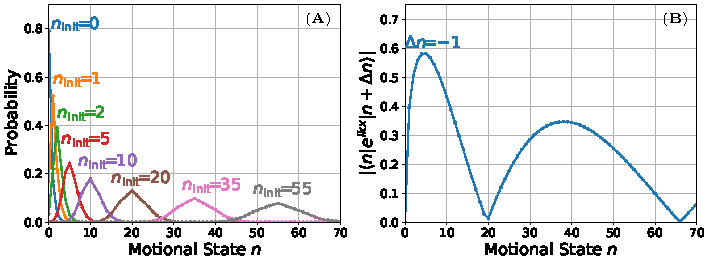
\includegraphics[width=\textwidth]{figures/na_rsc_challenges.pdf}
  \caption[Optical pumping motional-state redistribution and Raman coupling]{
    Optical pumping motional-state redistribution and Raman coupling for large LD parameters
    for the axial direction~($z$)~\cite{wineland_laser_1979}.
    The range plotted covers $95~\mathrm{\%}$ of the initial thermal distribution.
    (A) Motional state distribution after one OP cycle for different initial states motion,
    $n_{\textrm{init}}$.
    Due to photon-recoil and the large LD parameter, $\eta^{\textrm{OP}}_z=0.55$,
    there is a high probability of $n$ changing.
    (B) Matrix elements for Raman transition on the first order cooling sideband
    deviate from $\sqrt{n}$ scaling with multiple minima.
    \label{fig:rsc:na-challenges}}
\end{figure}

In our experiment, the OP Lamb-Dicke parameters are
$\eta^{\mathrm{OP}}_x, \eta^{\mathrm{OP}}_y, \eta^{\mathrm{OP}}_z = 0.25, 0.25, 0.55$.
Based on the metric above, any cooling sequences
that have fewer than $78~\mathrm{\%}$ cooling pulse for $z$~(axial) axis,
which is generally the case, should have a net cooling effect.
This, however, does not guarantee cooling into the ground motional state,
nor does it fully characterize the efficiency of the cooling sequence
since the averaging hides a few critical aspect of having a large Lamb-Dicke parameter.

One of the important effects can be seen in Fig.~\ref{fig:rsc:na-challenges}A showing
the motional state distribution after one OP cycle
for different initial motional states $n_{\mathrm{init}}$~\cite{wineland_laser_1979}.
Although the average heating is fixed at $4\omega_{\mathrm{recoil}}$,
independent of $n_{\mathrm{init}}$,
the spread or the uncertainty of $n$ after the OP is significantly
higher for high $n_{\mathrm{init}}$.
This effect significantly increases the difficulty in controlling the state during the
RSC sequence. It can negatively impact the cooling performance and
may lead to increased loss during cooling due to atom escaping to higher motional states.

The other important effect is the dependency of matrix element $M_{n,n+1}$
on the motional level $n$.
While this dependency is not a new effect, since the $\sqrt{n}$ dependency
on the cooling sideband strength exist even in the LD regime
and must be taken into account with
pulse time variation~\cite{wineland_experimental_1998,liu_molecular_2019}
to achieve efficient cooling, the high Lamb-Dicke parameter adds even more complications.
As shown in Fig.~\ref{fig:rsc:na-challenges}B, rather than a simple $\sqrt{n}$ dependency,
it is a non-monotonic function and more importantly has multiple minima, so-called ``dead-zone'',
within the range of motional states we are interested in~\cite{wineland_laser_1979}.
The coupling strength for states in the dead-zones can be reduced by more than ten times
which can significant affect the efficiency of the cooling pulse
and even makes it virtually impossible to drive Raman transitions on atoms in these states
in order to cool them further.
A cooling sequence can therefore accumulate pupolations in the dead-zones
rather than the ground state.
Their small coupling strength also reduce their signal level during
Raman sideband spectroscopy making these states nearly invisible to sideband thermometry
which further complicates the optimization of the cooling sequence.

\section{Solution: High Order Sidebands}
\label{ch:rsc:solution-high-orders}

\begin{figure}
  \centering
  \includegraphics[width=8cm]{figures/na_rsc_mele_raman.pdf}
  \caption[Raman coupling including high order sidebands]{
    Matrix elements for Raman transition including high order sidebands.
    During cooling, we utilize the fact that high motional states couple most effectively
    to sidebands with large $|\Delta n|$ in order to overcome the issue with
    variation and dead zone in the coupling strengths.
    \label{fig:rsc:na-mele-raman}}
\end{figure}

The main solution to the issues related to the large Lamb-Dicke parameter
is in fact the large Lamb-Dicke parameter itself.
The increased coupling to other motional state for large Lamb-Dicke parameter
and high motional states applies not only to $|\Delta n|=1$ but to higher $\Delta n$ as well.
Fig.~\ref{fig:rsc:na-mele-raman} shows the coupling to higher order cooling sidebands
which all have comparable strengths as the first order sidebands in different ranges
of motional states.

Because of this, it is now possible, and in some cases preferred, to apply Raman cooling pulse
on the higher order sidebands instead of only the first order one.
These pulses reduce more energy from the system per pulse which directly improves
the cooling to heating ratio and allows better control on the motional state
given the uncertainty after an OP pulse.
More importantly, depending on the motional level, there is always a sideband order
with significant coupling strength that can be used to cool it,
therefore completely removing the coupling dead-zones.
Moreover, by using each sideband orders only near their coupling maxima,
the coupling strength variation is also greatly reduced which removes
the need to vary the pulse times for all but the pulses on the first order sideband.

\section{Solution: Simulation Based Optimization}
\label{ch:rsc:simulation}

\begin{figure}
  \centering
  \includegraphics[width=\textwidth]{figures/na_rsc_sequence.pdf}
  \caption[Simulation optimized Raman sideband cooling sequence for Sodium]{
    Schematic of the cooling pulse sequence. The tweezer is strobed at 3 MHz to
    reduce light shifts during optical pumping~\cite{hutzler_eliminating_2017}.
    Each cooling cycle consists of $8$ sideband pulses.
    The four axial pulses address two sideband orders.
    The two pulses in each radial direction either address $\Delta n=-2$ and $\Delta n=-1$
    or have different durations to drive $\Delta n=-1$,
    at the end of the cooling sequence when most of the population is below $n=3$.
    The Raman cooling and spectroscopy pulses have Blackman envelopes~\cite{kasevich_laser_1992}
    to reduce off-resonant coupling,
    while the measurement Rabi pulses in Fig.~\ref{fig:rsc:na-rabi-flop}
    have square envelopes to simplify analysis.
    \label{fig:rsc:na-sequence}}
\end{figure}

The change in cooling technique by including higher order sidebands, however,
does not remove the effect of coupling variation on the sideband thermometry.
If a non-thermal distribution of motional states is produced by the cooling sequence,
the ratio of the first order sideband height still cannot be trusted to calculate
the temperature or the ground state probability.
Including higher order sidebands in the sideband thermometry could in principle
give us enough information about the state distribution but doing
so for a non-thermal distribution is not easy or reliable.
We therefore use a Monte-Carlo simulation to guide our search
for the optimal sequence~\cite{dalibard_wave-function_1992,chretien_laser_2014}.
The simulation includes accurate scattering rate and branching ratios
from the tweezer, Raman and OP beams.
For best simulation performance, the atom is assumed to be in a single motional state,
i.e. with a certain $n_x$, $n_y$ and $n_z$, after each Raman or OP step
\footnote{This assumes no coherence between different motional state,
  which is the case as long as each Raman pulses are separated from each other by OP pulses.}.
It is also assumed that each Raman pulse drives only the intended sideband order,
which is a property that needs to be ensured
in the experiment~(section~\ref{ch:rsc:implementation:pulse-shaping}).
For each cooling sequence simulated,
the Raman beam power and frequency, and the OP beam power and polarization purity
are varies slightly around the respective expected values
in order to confirm the robustness of the sequence against fluctuation in the experiment.
Fig.~\ref{fig:rsc:na-sequence} demostrate the resulting optimal sequence from the simulation.
In particular, we find that alternating the cooling pulses between two
neighboring orders for the axial direction and $\Delta n=-2$ and $\Delta n=-1$
for the radial directions
eliminates the accumulation of population in motional states with small Raman coupling.
The simulation also confirms that setting the coupling strength of each sideband
to drive a Rabi $\pi$-pulse corresponding to the maximum matrix element motional state
(i.e. the maxima in Fig.~\ref{fig:rsc:na-mele-raman}) yields efficient cooling, initially,
as we expected from section~\ref{ch:rsc:solution-high-orders}.
The efficiency of cooling on higher-order sidebands diminishes
as the atom approaches the ground state, so the final cycles utilize only
the $\Delta n=-1$ sideband while alternating between the three axes.

\section{Alignment of Raman and OP Beams}
\label{ch:rsc:alignment}

Due to small waist of the Raman beam, it is important to align the Raman beam to
the single atom with high precision in order to maximize the Raman Rabi frequency
as well as minimizing the intensity fluctuation of the Raman beam experienced by the atom
due to pointing instability.
Such precision cannot easily be achieved using external reference and
must be done by using the single atom itself as the alignment target.

In our experiment, we have developped two different methods to align or verify the alignment
of the Raman beams, both relying on the scattering from the Raman beams.
For initial alignment, or when the beam position is off-center
by more than a beam waist, we couple resonant Sodium D2 light into the Raman beam path
in order to enhance the scattering rate. The course alignment is done based on
maximizing depleting and displacement of the MOT due to radiation pressure.
After that, the fine alignment of the Raman beam is done by reducing the power in the Raman
beam path and maximizing the heating effect on the single atom.
When the Raman beam is focused on the tweezer position,
we can observe a depletion of the single atom live loading signal
while the MOT is not affected as significantly.
This process is then repeated with lower power in the Raman beam path until the desired
position sensitivity is reached.

\begin{table}
  \centering
  \caption[Na Raman beams parameters.]{
    Single photon Rabi frequency and scattering rate for the Na Raman beams.
    Since in general each beams couples to more than one excited states,
    the single photon Rabi frequency is listed for the reduced matrix element
    $\langle J=1/2||er||J'=3/2\rangle$~\cite{steck_sodium_2019}.
    The scattering is calculated for the $|F=2,m_F=2\rangle$ ground state
    since this is the dark state in the cooling scheme where the scattering matters the most.
    The polarization of the beams can be seen in Fig.~\ref{fig:rsc:na-geometry}.
    R5 is the F1 beam that is co-propagating with R3 with orthorgonal polarization
    that is used to drive sideband-free Raman transition (not used for cooling).
    We also assume $10~\mathrm{\%}$ power of the R1 beam is
    in the opposite circular polarization~($\sigma^+$) instead of being purely $\sigma^-$.
    \label{table:rsc:alignment:raman-parameter}}
  \begin{tabular}{|c|c|c|c|c|c|}
    \hline
    Beam&R1 (F2)&R2 (F1)&R3 (F2)&R4 (F1)&R5 (F1)\\\hline
    \makecell{Rabi Frequency\\($2\pi\times\mathrm{MHz}$)}&$41.2(23)$&$16.4(26)$&$45.5(31)$&$34.8(21)$&$41.4(26)$\\\hline
    \makecell{Scattering Rate\\($2\pi\times\mathrm{Hz}$)}&$5.41(62)$&$1.50(48)$&$11.0(15)$&$6.74(82)$&$9.5(12)$\\\hline
  \end{tabular}
\end{table}

\todo{appendex about scattering branching ratio calculation}
In order to verify the alignment of the tweezer without any physical change to the beam path,
we use a second method to calibrate the single photon Rabi frequency of the Raman light.
This method requires a working OP to initialize the spin state of the atom
so it is less convenient for aligning from scratch.
To use this method, the atom is first loaded in the tweezer and initialized
in the $|2,2\rangle$ state. We then turn on a single Raman beam at maximum power for a
variable length of time. The off resonance scattering from the Raman beam will cause
the spin state of the atom to change and the population in $F=1$ state is measured
by removing the $F=2$ population using a pushout pulse.
The rate of the spin change is fitted to a theory model to derive the Rabi frequency of
the Raman light.
The result of the fit is shown in table.~\ref{table:rsc:alignment:raman-parameter}.
The table also includes the total scattering rate from each Raman beams
which corresponds to a cumulative $3$ scattering event
on average during the whole cooling sequence and
should not be a limiting factor for the cooling performance.

The OP beam has a much larger waist~($\approx\!1~\mathrm{mm}$)
and therefore require less alignment in the beam position.
However, since the OP beam needs to be on resonant with the excited state,
the strong light shift from the tweezer can significantly affect the OP efficiency.
Fortunately, the method described in section~\ref{ch:loading:loading}
that fixes this problem for the loading of the atom in the tweezer can also be used here.
In this case, however, only the tweezer light is being switched on and off at $2.5~\mathrm{MHz}$
and not the OP light for simplicity.
Due to the low intensity and Rabi frequency of the OP light,
the OP will be completely stopped during the on-cycle of the tweezer
causing the OP to happen only during the off-cycle when there is zero light shift.

In order to take advantage of the dark state optical pumping and
minimize unnecessary scattering for atoms in the $|2,2\rangle$ state,
the OP beam need to have a pure $\sigma^+$ polarization.
This requires the OP beam to propagate parallel to the magnetic field
in additional to having the currect circular polarization.
The alignment is done by minimizing ``depumping'' of the atom spin state caused by the OP beam,
similar to the technique we used to calibrate the Raman beam Rabi frequency.
After the atom is initialized in the $|2,2\rangle$ state, we turn on the D1 OP light
for a certain time which should not address the atom when perfectly aligned.
The misalignment of the beam, however, will cause the atom to scatter from the OP beam
and change to $F=1$ state, i.e. ``depumped'', with certain probability.
We then change the alignment of the beam an minimize the depumping rate.
Due to a similar requirement for Cesium OP, the probagation direction of
the OP beam for Sodium and Cesium are aligned to each other by overlapping them
using mechanical target to better than $0.08^\circ$ first
before the magnetic field direction is aligned to the OP beams by minimizing depumping.
For polarization alignment, we first clean up the linear polarization of the light
using the LPVISC050-MP2  nanoparticle linear film polarizer from Thorlabs
with better than $100,000:1$ extinction ratio.
After that we use both a half waveplate and a quater waveplate
to generate a circularly polarized light.
We observed that both the polarization cleanup and the half waveplate is necessary
to obtain the best polarization alignment in order to compensate for the polarization
fluctuation caused by the fiber as well as the birefringence of the optics and windows
within the OP beam path. After alignment, the OP intensity is calibrated
by measuring the OP rate for atom prepared in $|2,1\rangle$ state
using Raman transitions\footnote{One from $|2,2\rangle$ to $|1,1\rangle$
  and a second one from $|1,1\rangle$ to $|2,1\rangle$.}.
From this measurement we determined that the power impurity of the OP polarization
to be $\approx\!100~\mathrm{ppm}$.

Other than the alignment procedure above, we have also observed that reflection
of the OP beam can contribute significantly to the polarization impurity and
must be avoided. In particular, since the Raman beam R1 counter propagate with the OP beam,
it is possible for the OP beam to be coupled into the Raman fiber and then retro-reflected
to be focused onto the atom through the Raman beam path at a wrong polarization.
Since the Raman beam size is much smaller, we have observed as much as $3~\mathrm{\%}$
polarization impurity caused by this mechanism despite only a small amount of
power being reflected. This issue, along with other reflections,
are reduced by avoiding optics with normal incident on the exit path of the OP beam
as well as changing the propagation direction of the R1 Raman beam
to have a small angle with the OP beam which reduces the OP power coupled into
the Raman beam fiber.

\section{Implementing Optimized RSC Sequence}
\label{ch:rsc:implementation}

In order to achieve the optimal cooling performance, a few more considerations are important
for implementing the sequence from section~\ref{ch:rsc:simulation}.

\subsection{Pulse shaping}
\label{ch:rsc:implementation:pulse-shaping}

In order to achieve optimal performance from the cooling sequence,
it is important to accurately drive the intended sideband order.
In fact, in the absense of undesired scattering,
the frequency resolution of the Raman transition limits the lost achievable temperature.
This is particularly important when driving the first order cooling sidebands
since any coupling to the carrier may change the spin state of the atom without
removing any motional energy therefore causing a net heating effect after the OP pulse.

The obvious way to achieve this is to narrow the linewidth of the Raman transition,
e.g. by using a lower power or Raman Rabi frequency.
However, reducing the lineiwth of the transition also increase the susceptibility
to resonance fluctuation.
Therefore the desired solution is to reduce the off-resonance coupling of the Raman beam
for large detuning while increasing or maintaining the coupling for small detuning.
We achieve this by using a Blackman pulse shape for
the Raman transition~\cite{kasevich_laser_1992}.
\footnote{While more complex pulses can be constructed
  to achieve a even sharp detuning cutoff~\cite{fu_broadband_1995},
  such pulses generally significantly increases the pulse time
  and can cause more heating during cooling due to scattering and other heating mechanisms.
  The Blackman pulse we use offers a balance between the pulse time
  and off-resonance coupling reduction.}

\subsection{Calibration}
\label{ch:rsc:implementation:calibration}

The Raman sideband frequencies are calibrated by measuring the Raman spectrum before cooling
(an example of which is shown in the initial spectrum in Fig.~\ref{fig:rsc:na-spectrum}).
However, since high sideband orders are mainly used to cool atoms in high motional state,
the resonance frequency for these sideband are not equal spacing anymore due to
the anharmonicity of the trap.
In order to estimate the effect on the sideband frequencies,
we can define anharmonicity as $A_{i,n}=(E_{i,n+1}-E_{i,n})/h - \omega_i/(2\pi)$
for each trap axis $i$, and calculated from the quartic term
of the optical tweezers via perturbation theory.
In the paraxial approximation, we find $A_{i,n}=-3n\hbar/4\pi m d_i^2$,
where $d_i$ equals the beam radius for the radial directions and
$d_z\approx\pi w_{0,x}w_{0,y}/\lambda_{\textrm{trap}}$.
Numerically, $\{A_{x,n},A_{y,n},A_{z,n}\}=\{-1.4, -1.4, -0.16\}n~\mathrm{kHz}$.
For the states addressed by high order sidebands,
this broadens and shifts high-order sidebands
due to the $n$-dependence of the transitions.

To mitigate this, we calibrate the frequency of each sideband order individually
at the initial temperature. However, since the first order sideband is mainly used to cool atoms
that are closed to the ground state,
their resonance frequency  is recalibrated using partially cooled atoms after the initial calibration.
The use of high Rabi frequency and Blackman pulse shape also reduces the effect
of anharmonicity by broadening the spectrum as much as possible.

Although we can calibrate the single photon Rabi frequency of the Raman beams from
the scattering rate~(section~\ref{ch:rsc:alignment}),
we also calibrate the Raman Rabi frequency on the carrier and different sideband orders.
This offers a more direct and sensitive measurement for the cooling sequence parameter.
Unlike resonance frequency, the anharmonicity only has a second order effect on the Rabi frequency
and is therefore ignored. The calibration measures
only the carrier and first order heating sideband which has the highest signal after cooling
(an example of which is shown in the cooled Rabi flopping signal in
Fig.~\ref{fig:rsc:na-rabi-flop}).
The Raman Rabi frequencies measured on these two transitions are used to calculate
the full Rabi frequency $\Omega_{\mathrm{R}}^0$ and the Lamb-Dicke parameter,
which are in-turn used to calculate the Rabi frequency on other sideband orders.

Since the final calibration of both the Raman Rabi frequency and resonance requires a working
cooling sequence, when optimizing the sequency from scratch,
the calibration process is applied iteratively as the cooling performance is improved.

\section{Cooling Performance}
\label{ch:rsc:performance}

\begin{figure}
  \centering
  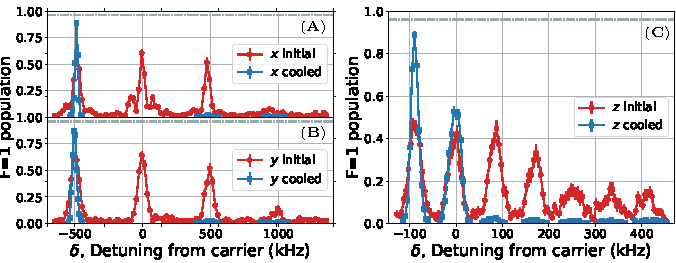
\includegraphics[width=\textwidth]{figures/na_rsc_spectrum.pdf}
  \caption[Raman sideband spectra before and after cooling]{
    Raman sideband spectra for (A) $x$, (B) $y$, (C) $z$ axis before (red circle)
    and after~(blue square) applying Raman sideband cooling sequence.
    The height of the cooling sidebands~(positive detuning)
    are strongly suppressed after cooling which suggests most of the atoms are cooled
    to the motional ground state in the trap.
    \label{fig:rsc:na-spectrum}}
\end{figure}

\begin{FPfigure}
  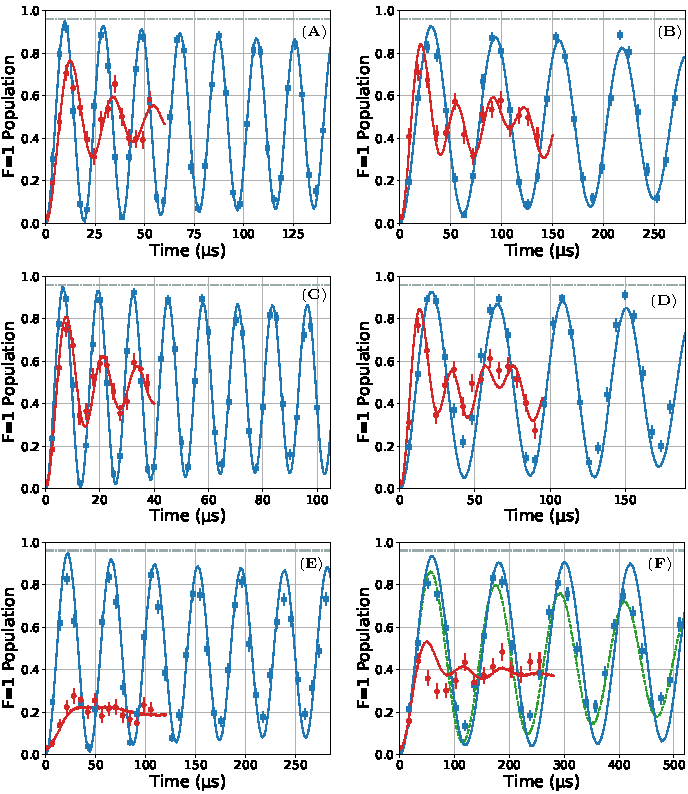
\includegraphics[width=\textwidth]{figures/na_rsc_rabi_flop.pdf}
  \caption[Rabi flopping on carriers and sidebands]{
    Rabi flopping on radial axis $x$ (A) carrier and (B) $\Delta n_x=1$ sideband,
    radial axis $y$ (C) carrier and (D) $\Delta n_x=1$ sideband,
    axial axis $z$ (E) carrier and (F) $\Delta n_x=1$ sideband,
    before~(red circle) and after~(blue square) Raman sideband cooling.

    Solid lines (both red and blue) in all plots are fits to a Rabi-flopping
    that includes a thermal distribution of motional states~\cite{meekhof_generation_1996}
    as well as off-resonant scattering from the Raman beams.

    The blue lines correspond to a ground state probability of
    (A-D) $98.1~\mathrm{\%}$ along radial axis
    and (E-F) $95~\mathrm{\%}$ along the axial axis after cooling.
    The red lines correspond to a thermal distribution of $80~\mathrm{\mu K}$ before RSC.
    The horizontal dashed lines in all the plots correspond to the $4~\mathrm{\%}$ probability
    of imaging loss.

    The green dashed line in (F) includes the additional decoherence due to
    a fluctuation of the hyperfine splitting of magnitude $3~\mathrm{kHz}$.
    We see that the decoherence effect is strongest for the post-cooling data on
    the axial $\Delta n_z=1$ sideband where the Rabi frequency is the lowest.
    \label{fig:rsc:na-rabi-flop}}
\end{FPfigure}

Our final cooling results are shown in Fig.~\ref{fig:rsc:na-spectrum} and
\ref{fig:rsc:na-rabi-flop}.
In total, $540$ cooling pulses (total duration $53~\mathrm{ms}$) are applied
along three axes with cooling beginning on the radial second order and axial fifth order.
The full sequence including calibrated parameters can be found in appendix~\ref{appendex:rsc}.

For the more tightly confined radial directions,
we observe clear $\Delta n=1$, $\Delta n=-1$, and $\Delta n=-2$ sidebands before RSC,
as is shown in Fig.~\ref{fig:rsc:na-spectrum}A and B.
After RSC, the $\Delta n=-1$ and $\Delta n=-2$ sidebands
on both radial axes are strongly reduced.
Using Eq.~\ref{eq:rsc:thermometry:p0} and \ref{eq:rsc:thermometry:nbar},
we obtain $\bar{n}_x=0.019(4)$ and $\bar{n}_y=0.024(3)$ from the spectrum which
correspond to ground-state fractions of $98.1(5)~\mathrm{\%}$ and $97.6(3)~\mathrm{\%}$,
in agreement with fitted values of $98(1)~\mathrm{\%}$ and $95(3)~\mathrm{\%}$
from the Rabi flopping curves~\cite{meekhof_generation_1996}
in Fig.~\ref{fig:rsc:na-rabi-flop}A-D.
The initial temperature of $80~\mathrm{\mu K}$ before RSC is obtained from similar fits.

For the weak axial direction
where cooling is challenging because the atom starts outside the LD regime,
we observe up to $5$th-order Raman cooling sidebands initially,
which indicates population in highly-excited motional states.
Nevertheless, our cooling sequence works efficiently
as all the $\Delta n<0$ sidebands are reduced after RSC~(Fig.~\ref{fig:rsc:na-spectrum}C).
Using the ratio of first-order sideband heights, we obtain $\bar{n}_z=0.024(5)$,
which corresponds to a ground state population of $97.6(5)~\mathrm{\%}$,
in agreement with a ground state population of $95(4)~\mathrm{\%}$ extracted from Rabi flopping
when $\Delta n=0$~(Fig.~\ref{fig:rsc:na-rabi-flop}E).
For the $\Delta n=1$ sideband~(Fig.~\ref{fig:rsc:na-rabi-flop}F),
we observe additional decoherence that is more pronounced due to the slower Rabi frequency.
The decoherence rate is consistent with magnetic field fluctuations of $1.5~\mathrm{mG}$
measured independently in the lab, which would produce a Zeeman shift of $\sim 3~\mathrm{kHz}$.

Combining the axial and radial cooling results,
a single Na atom is in the 3D ground state with a probability of $93.5(7)~\mathrm{\%}$ after RSC.
The cooling efficiency is limited by spontaneous scattering rate~($0.1-0.2~\mathrm{kHz}$)
from the Raman beams, as well as spectral broadening from magnetic field fluctuations.

We measure a heating rate that corresponds to decreasing 3D ground state population
at a rate of $\sim0.9~\mathrm{\%/ms}$.
The rate is consistent with off-resonant scattering of
the trapping light~\cite{grimm_optical_2000},
and is predominantly in the axial direction where the trapping beam propagates.

Monte-Carlo simulations show that the ground state probability after RSC
could be enhanced by increasing the detuning of the Raman beams and implementing
better control of the magnetic field. Another improvement could come from
grey molasses cooling,
to achieve a lower starting temperature before RSC~\cite{colzi_sub-doppler_2016}.

\section{Summary and Outlook}
\label{ch:rsc:summary}

We have shown that despite the difficulty in achieving a low optical cooling temperature
of low mass sodium atoms, three dimensional cooling
with significant ground state population can be achieved
by using high-order Raman sidebands in an optimized cooling sequence.
The challenges we face with the cooling of Na atom is shared with
a large variety of other systems including exotic atoms and molecules,
where the initial temperature and available trapping potential may be limited.
The techniques we used are well-suited for these systems
and open up a route to ground state cooling.

In our experiment, the RSC step concludes our full control of the atom quantum states.
The atoms are then merged into the same trap adiabatically
so that they remains in a single quantum state~\cite{liu_molecular_2019}.
This is the starting point for our study of
the atom-atom interaction and molecular potentials,
as well as the coherent formation of molecules.
These will be the focus of the following chapters.
